\documentclass[a4paper, DIV=15]{scrartcl}
\usepackage{grawlix}
\usepackage{pullquote}
\usepackage{graphicx}
\usepackage{multicol}
\usepackage{enumitem}
\usepackage{lipsum}

\tolerance=1
\emergencystretch=\maxdimen
\hyphenpenalty=10000
\hbadness=10000

\setkomafont{section}{\setmainfont{Quicksand-Bold}\Large}

% Adjust spacing before and after section headings
\RedeclareSectionCommand[
  runin=false,
  afterindent=false,
  beforeskip=0.5\baselineskip,
  afterskip=0.25\baselineskip,
]{section}

% Adjust spacing before and after subsection headings
\RedeclareSectionCommand[
  runin=false,
  beforeskip=0.5\baselineskip,
  afterskip=-0.25\baselineskip
]{subsection}

% Adjust spacing before and after subsubsection headings
\RedeclareSectionCommand[
  runin=false,
  beforeskip=0.5\baselineskip,
  afterskip=-0.25\baselineskip
]{subsubsection}

%\raggedright
\begin{document}

\thispagestyle{empty}
\enlargethispage{3.5\baselineskip} % Move the bottom line (author and date) down a bit


{
\begin{center}
\setmainfont[Scale=3.0]{Cooper Black}
\Huge
Grawlix
\end{center}
}
{
\begin{center}
\setmainfont{Quicksand-Medium}
\noindent{}\Large{}by Michael Purcell and Dannielle Harden\\grawlix.board.game@gmail.com
\end{center}
}

\smallskip
\begin{multicols}{2}
\section*{Overview}
Grawlix is an abstract strategy game for two players that can be played in 15\textendash 30 minutes. It is suitable for all ages, but is intended for players who are eight years old or older.

\section*{Components}
Grawlix is played with a set of thirty-six tiles. There is one tile for each possible combination of six punctuation marks and six colors.

\section*{Gameplay}
Grawlix is a version of the typesetters' game (see below). The players take turns playing tiles, creating a rectangular grid that grows over the course of the game.

\section*{Objective}
The winner is the player who is able to force their opponent into a position where they have no legal moves remaining.
\end{multicols}

\begin{center}
\begin{tikzpicture}[transform shape, scale=2.33]
\node[tile, rotate=-30] () at (-2.5,0) {};
\pic[rotate=-30] () at (-2.5,0) {at={red}};

\node[tile, rotate=15] () at (-1.5,0) {};
\pic[rotate=15] () at (-1.5,0) {octothorpe={orange}};

\node[tile, rotate=-15] () at (-0.5,0) {};
\pic[rotate=-15] () at (-0.5,0) {dollar={yellow}};

\node[tile, rotate=15] () at (0.5,0) {};
\pic[rotate=15] () at (0.5,0) {percent={green}};

\node[tile, rotate=-15] () at (1.5,0) {};
\pic[rotate=-15] () at (1.5,0) {ampersand={blue}};

\node[tile, rotate=30] () at (2.5,0) {};
\pic[rotate=30] () at (2.5,0) {asterisk={violet}};

\end{tikzpicture}
\end{center}

\vspace{-1cm}

\setkomafont{section}{\setmainfont{Quicksand-Bold}\Large\center}
\section*{The Typesetters' Game}
\begin{pullquote}
{object={
%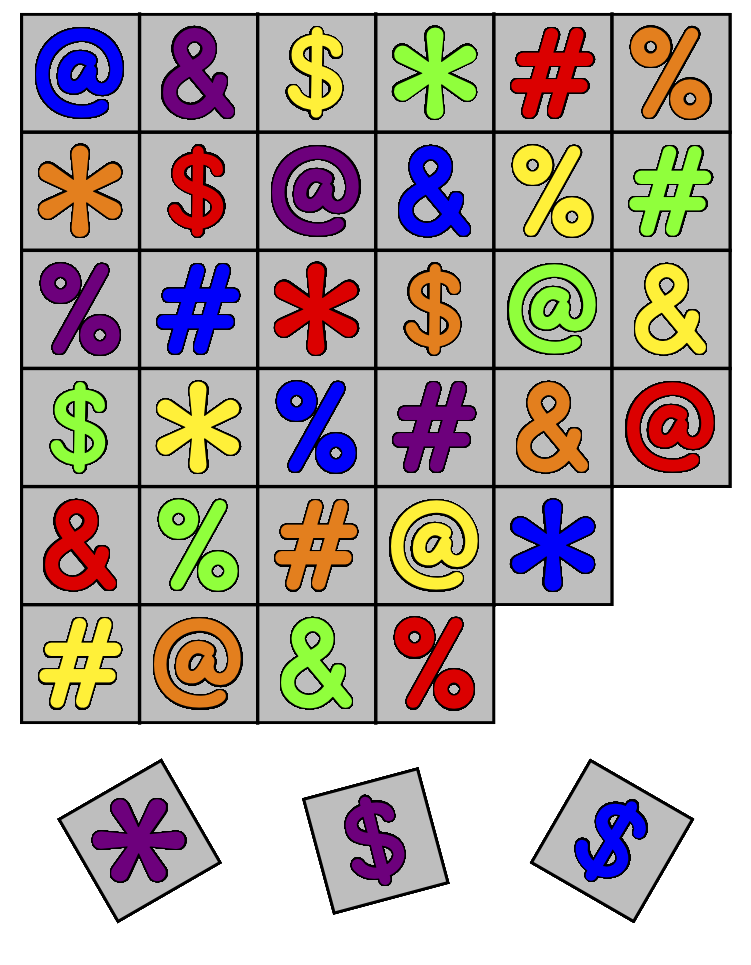
\includegraphics[scale=0.2]{Images/cover_image.png}},
\begin{tikzpicture}[transform shape, scale=2.33]
\foreach \i/\j/\k in {0.0/blue/at, 0.5/violet/ampersand, 1.0/yellow/dollar, 1.5/green/asterisk, 2.0/red/octothorpe, 2.5/orange/percent} {
	\node[tile] () at (\i,0.0) {};
	\pic () at (\i,0.0) {\k={\j}};
}

\foreach \i/\j/\k in {0.0/orange/asterisk, 0.5/red/dollar, 1.0/violet/at, 1.5/blue/ampersand, 2.0/yellow/percent, 2.5/green/octothorpe} {
	\node[tile] () at (\i,-0.5) {};
	\pic () at (\i,-0.5) {\k={\j}};
}

\foreach \i/\j/\k in {0.0/violet/percent, 0.5/blue/octothorpe, 1.0/red/asterisk, 1.5/orange/dollar, 2.0/green/at, 2.5/yellow/ampersand} {
	\node[tile] () at (\i,-1.0) {};
	\pic () at (\i,-1.0) {\k={\j}};
}

\foreach \i/\j/\k in {0.0/green/dollar, 0.5/yellow/asterisk, 1.0/blue/percent, 1.5/violet/octothorpe, 2.0/orange/ampersand, 2.5/red/at} {
	\node[tile] () at (\i,-1.5) {};
	\pic () at (\i,-1.5) {\k={\j}};
}

\foreach \i/\j/\k in {0.0/red/ampersand, 0.5/green/percent, 1.0/orange/octothorpe, 1.5/yellow/at, 2.0/blue/asterisk} {
	\node[tile] () at (\i,-2.0) {};
	\pic () at (\i,-2.0) {\k={\j}};
}

\foreach \i/\j/\k in {0.0/yellow/octothorpe, 0.5/orange/at, 1.0/green/ampersand, 1.5/red/percent} {
	\node[tile] () at (\i,-2.5) {};
	\pic () at (\i,-2.5) {\k={\j}};
}
\end{tikzpicture}},
shape=rectangular}
A pair of typesetters once worked for a local newspaper. Every Sunday, they produced a set of comic strips. This was challenging because it was so different from their regular work. In particular, the cartoonists sometimes used strings of punctuation to replace profanity. The typesetters often had to improvise to find enough type to print those sections. So, they set aside the type that they used for this purpose in a special case. Over time, they amassed a collection of thirty-six pieces of type. They had one for each of six punctuation marks in each of six typefaces.

One day, while they were setting that week's comics, they noticed a curious phenomenon. They had arranged their collection of type in a square on their workbench. It was easy to ensure that every row and column had only one of each punctuation mark. It was easy to ensure that every row and column had only one of each typeface. Despite their best efforts, they could not find a way to do both at the same time.

They turned this puzzle into a game that they could play as they worked. Both players would grab a handful of type at the beginning of the day. Then, they would take turns playing by placing those pieces on the workbench. They had to place each piece next to a piece that had been played earlier. This created a grid of tiles that grew as they played. Each row and column of the grid could have only one of each punctuation mark and one of each typeface. The grid could have no more than six rows and six columns.

The game continued in this way until one player was unable to find a legal move. That player would be the loser of the game and would have to come in a few minutes early the next morning to make coffee.

\end{pullquote}
\end{document}